\documentclass{article}[18pt]
\usepackage[utf8]{inputenc}
\usepackage[margin=0.7in]{geometry}
\usepackage{parselines} 
\usepackage{amsmath}
\usepackage{titlesec}
\usepackage{pgfplots}
\usepackage{graphicx}
\usepackage[english]{babel}
\usepackage{fancyhdr}
\usepackage{circuitikz}
\pgfplotsset{width=10cm,compat=1.9}

\titlespacing\section{0pt}{14pt plus 4pt minus 2pt}{0pt plus 2pt minus 2pt}
\newlength\tindent
\setlength{\tindent}{\parindent}
\setlength{\parindent}{0pt}
\renewcommand{\indent}{\hspace*{\tindent}}

\pagestyle{fancy}
\fancyhf{}
\rhead{Sam Robbins 13SE}
\lhead{A Level Physics - Fields}
\rfoot{Page \thepage}


\begin{document}
\begin{center}
\underline{\huge Capacitors}
\end{center}
A capacitor is constructed from two conducting plates separated by an insulator.\\
Charge can flow onto and off the plates but not across the plates.

\section{Charging circuit for a capacitor}
\begin{center}
\begin{circuitikz}[american voltages]
\draw
  (0,0) to [short] (3,0)
  to [battery] (4,0)
  (4,0) to[short] (5,0)
  (4.4,-3) node[spdt](spdt) {}
  (5,0) to[short] (spdt.out 1)
  (spdt.in) to [capacitor] (2,-3)
  (2,-3) to[short] (0,-3)
(0,-3) to[short] (0,0)
(spdt.out 2) to [short] (5,-5) 
(5,-5) to[lamp] (1,-5) 
(1,-5) to[short] (0,-5)
(0,-5) to[short] (0,-3)
  ;
  \end{circuitikz}
  \end{center}
  
When charging the current flows round the top half of the circuit, when discharging the SPDT is changed to the other output and the current flows round the bottom half of the circuit.\\
\\
Capacitors can be used as simple timers in circuits.
\\
\\
The time it takes to charge/discharge depends on:
\begin{itemize}
\item The capacitance of the capacitor \textbf{(C)}
\item The resistance of the charging/discharging circuit \textbf{(R)}
\end{itemize}
\section{Energy stored in a capacitor}
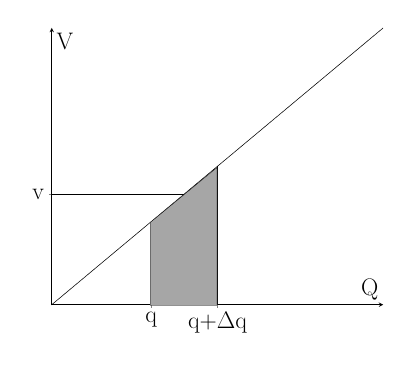
\begin{tikzpicture}[scale=0.5]
\begin{axis}[xmin=0,ymin=-0.01,ylabel=V,xlabel=Q,axis lines=middle,label style={font=\LARGE},
ytick={2},yticklabels=v,
ticklabel style = {font=\LARGE},
xtick={1.5,2.5},xticklabels={q,q+$\Delta$q}
]
\addplot[mark=none]{x};
\addplot [mark=none] coordinates {(1.5,0) (1.5, 1.5)};
\addplot [mark=none] coordinates {(2.5,0) (2.5, 2.5)};
\addplot[mark=none,domain=0:2]{2};
\end{axis}
\filldraw[black, ultra thin,fill=gray!70] (2.5,0) -- (4.2,0) -- (4.2,3.5) -- (2.5,2.1) -- cycle;
\end{tikzpicture}\\
Area under graph=work done\\
V is the average P.D. as charge increases from q to q+$\Delta$q\\
$\Delta \text{w=v}\Delta \text{q}$\\
\\
$Q=\frac{1}{2}QV=E$  \textbf{(Work done=energy stored)}\\
\\
How to answer the exam question: Show that the energy stored by a capacitor is given by $E=\frac{1}{2}QV$
\begin{enumerate}
\item Sketch a graph of Q against V and describe what it shows
\item Describe that electrical energy is the product of charge and voltage
\item State QV is represented by the area under the line
\item The area under the line is a triangle with area =$\frac{1}{2}QV$
\item Therefore $E=\frac{1}{2}QV$
\end{enumerate}
$E=\frac{1}{2}QV$\\
$Q=CV$\\
Therefore:\\
$E=\frac{1}{2}CV^2$\\
$E=\frac{1}{2}\dfrac{Q^2}{C}$\\
\\
The battery supplies energy QV to the circuit but the capacitor only stores $\frac{1}{2}QV$, this means that 50\% of the energy provided by the battery is wasted due to resistance in the circuit.

\end{document}